\chapter{Fundamentos te\'oricos}\label{capit:cap2}
\vspace{-2.0325ex}%
\noindent
\rule{\textwidth}{0.5pt}
\vspace{-5.5ex}% 
\newcommand{\pushline}{\Indp}% Indent puede ir o no :p

\section{Introducci\'on}\label{secc:introduccion}
La ansiedad es un fen\'omeno que solemos experimentar en algunas situaciones de nuestras vidas, como  al dar un discurso en p\'ublico, al ser entrevistado para un nuevo trabajo o durante un examen. Nos ayuda a mantenernos alertas y listos para enfrentar las situaciones que se viven diariamente. La ansiedad es un estado mental en el que experimentamos sentimientos de preocupaci\'on, nerviosismo o, incomidad, t\'ipicamente asociada a un evento inminente o incierto. Un sector de la poblaci\'on afectada por la ansiedad es el de los cuidadores de personas con demencia. En este cap\'itulo se define la ansiedad, como se origina y afecta a los cuidadores y como podemos medirla por medio de instrumentos de auto reportado.

\section{Qu\'e es la Ansiedad?}\label{secc:ansiedad}

	La ansiedad es una emoci\'on caracterizada por sensaciones de tensi\'on, pensamientos de preocupaci\'on y cambios f\'isicos como incremento en la presi\'on arterial \citep{psychologyapa}, aumento de la sudoraci\'on y palpitaciones, entre otras respuestas fisiol\'ogicas. Estas manifestaciones se dan en determinados lapso de tiempo durante la vida del individuo. Durante estos lapsos, se dice que el sujeto se encuentra en un estado mental de ansiedad. Este estado mental es \'util para los humanos debido a que la ansiedad es una reacci\'on normal del cuerpo para lograr objetivos o lograr sobrevivir ante a una amenaza. Sin embargo, cuando la persona experimenta un nivel tan alto de ansiedad que no le permite manejar su vida normal, se dice que la persona tiene un desorden de ansiedad \citep{repetto2013}. 

\subsection{Ansiedad y estr\'es}\label{secc:anxietyandstress}
Si bien, en ocasiones el estr\'es y la ansiedad son conceptos que se usan de manera intercambiable, existen diferencias entre ambos. El estr\'es es definido como el desbalance entre la carga mental dada y la percepci\'on de las habilidades que el individuo tiene para lidiar con dicha carga. Este desbalance puede hacer que la ansiedad aumente, mientras que la ansiedad puede a su vez generar estr\'es. %La relaci\'on entre el estr\'es y la ansiedad es que la ansiedad es la se\~nal psicofisiol\'ogica de que la respuesta al estr\'es ha sido iniciada \citep{PMID2235645}.


\subsection{Ansiedad situacional y Ansiedad como rasgo}\label{secc:anxieystatevstrait}
Existen dos clasificaciones de ansiedad reconocidas por la \textit{American Psychological Association} \citep{psychologyapa} , las cuales se describen a continuac\'on.

\begin{itemize}
	\item{\textbf{Ansiedad situacional:}} Es una manifestaci\'on de ansiedad acerca de un evento \textbf{presente} bien definido. Normalmente la persona se encuentra conciente de la fuente de su ansiead. 
	\item{\textbf{Ansiedad como rasgo:}} Es una manifestaci\'on a largo plazo de la ansiedad, en la que el individuo puede entrar al estado ansioso sin saber la raz\'on que lo provoca. Las personas con personalidades t\'imidas tienden a sufrir mas de este tipo de ansiedad.

\end{itemize}

A pesar de que los efectos negativos en la calidad de vida de las personas que sufren de ansiedad como rasgo son mas fuertes que en la ansiedad situacional, este trabajo est\'a enfocado en la ansiedad situacional. Detectar estas situaciones podr\'ia brindar una posibilidad al cuidador de manejar su ansiedad adecuadamente.
\section{Demencia}\label{secc:dementia}
La demencia es un s\'indrome del declive de las habilidades cognitivas. Los s\'intomas comunes son: problemas de memoria, dificultades para realizar actividades de la vida diaria (como afeitarse, lavarse los dientes y cambiarse de ropa)\footnote{Activities of Daily Life (ADL)}, mal juicio, deterioro del lenguaje hablado y cambios de humor \citep{Aziz}. Afecta a alrededor del 4\% de las personas mayores de 65 a\~nos y al 40\% de las personas mayores de 90. La demencia suele manifestarse en s\'indromes como el de Alzheimer. Las personas con demencia en las fases CDR-3 o posterior necesitan de una persona que cuide de ellos \citep{meuser2001comprehensive}, normalmente durante el resto de su vida. Usualmente necesitan ayuda en las actividades de la vida diaria, siendo esto una carga para los cuidadores.

\section{Cuidadores}\label{secc:caregivers}
Uno de los sectores de poblaci\'on vulnerable, es el de los cuidadores de personas con demencia. Se encuentra documentado que los cuidadores, al llevar una carga f\'isica, cognitiva, y emocional derivada de su labor les genera padecimientos como ansiedad, estr\'es, y hasta la muerte \citep{Chen2013} debido a sobrecargas f\'isicas, debilitamiento del sistema inmunol\'ogico y riesgos de enfermedades del coraz\'on. En un estudio, cuidadores que sufren de ansiedad relacionada con la actividad de cuidador reportaron un 63\% de taza de mortalidad mayor que los no cuidadores de la misma edad \citep{bonsang282shulz}. Debido a que los cuidadores no necesariamente son personas con una formaci\'on profesional, pueden sufrir m\'as los efectos de ansiedad. Por lo general, los cuidadores que son familiares del paciente son a\'un m\'as afectados ya que necesitan administrar el tiempo de trabajo, familia, actividades sociales y la actividad propia del cuidado del paciente.
			%Cuales son las situaciones ( escenarios ) en los que los CUIDADORES presentan ansiedad?

\subsection{C\'omo se genera la ansiedad en los cuidadores?}\label{secc:caregiverburden}

\begin{figure}[h]
	\centering
	\subfigure[]{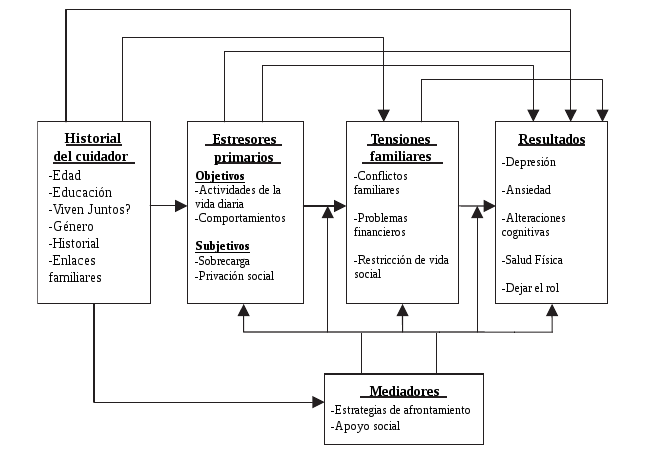
\includegraphics[width=180mm,height=120mm,keepaspectratio]{./Figures/anxiety_caregiver}} 
	\caption{El modelo de ansiedad en cuidadores (Pearlin et. al 1990)} \label{fig:modeloAnsiedad}
\end{figure}
El modelo de la ansiedad en cuidadores, es definido por Pearlin como un conjunto de caracter\'isticas que incluye el historial del cuidador, estresores primarios, tensiones familiares y estrategias de afrontamiento, las cuales tienen como salida efectos positivos o negativos\citep{Pearlin01101990}. A continuaci\'on, se explica el modelo de Pearlin elemento por elemento.
	\subsection{Historial del cuidador}{\label{secc:modeloAnsiedadCaregivers}}
		La edad, g\'enero, el nivel de educaci\'on y los lazos que tiene el cuidador con la persona con demencia son los principales factores que pueden hacer mas suceptible a los cuidadores de sufrir los efectos de la ansiedad. Por ejemplo, un adolescente sin experiencia de cuidador podr\'ia sentirse en grandes aprietos al tratar de satisfacer una necesidad de una persona con demencia. De la misma forma es emocionalmente dif\'icil para los cuidadores ver como el declive cognitivo de un familiar con demencia se va desarrollando hasta el grado de que no reconocer a sus propios hijos.
	\subsection{Estresores primarios}{\label{secc:modeloAnsiedadStressFactors}}
		Los factores de estr\'es primarios, o la carga f\'isica y/o cognitiva se dividen en dos: Objetivos y subjetivos. Los objetivos son aqu\'ellos que son cuantificables como las actividades la vida diaria y los comportamientos de la persona con demencia. Estos los podemos medir de acuerdo a la frecuencia y severidad de los eventos en un espacio de tiempo y podemos hacer un registro de ellos. Por otra parte, los subjetivos son aqu\'ellos que afectan a la percepci\'on del cuidador: Sobrecarga cognitiva y privaci\'on social.
	\subsection{Tensi\'ones familiares}{\label{secc:modeloAnsiedadSecondaryroles}}
		Comunmente los cuidadores son familiares que viven en la misma casa que la persona con demencia por lo que suelen tener diferentes roles sociales. Muchos de ellos son madres, padres, o hijos que tienen la obligaci\'on de trabajar y proveer de recursos al hogar. La carga extra de cuidar a una persona con demencia puede resultar en un desequilibrio emocional del cuidador.
	
	\subsection{Estrategias de afrontamiento}{\label{secc:modeloAnsiedadCoping}}
	Algunos cuidadores logran reducir su nivel de ansiedad por medio de estrategias de afrontamiento. Ejercicios de respiraci\'on, la b\'usqueda de apoyo de familiares y amigos o el consuelo religioso son algunas de las t\'ecnicas que son de mayor utilidad a los cuidadores \citep{Sharma20121287}.  Sin embargo, no todos ellos las utilizan o utilizan estrategias negativas como el uso de alcohol o drogas.

	Las consecuencias en el modelo de Perlin son los niveles de depresi\'on, ansiedad, y salud f\'isica del cuidador. El buen uso de las estrategias de afrontamiento, el balance de roles, y carga del cuidador pueden ayudar a reducir su ansiedad y mejorar su salud f\'isica y/o mental.

	\subsection{Cuidadores formales e informales}\label{secc:caregivers}
		Existen dos tipos de cuidadores: Formales e informales. Los cuidadores formales son aqu\'ellos que se encuentran afiliados con un sistema de servicio formal. Pueden recibir un pago o ser personas voluntarias. Mientras que los cuidadores informales son familiares, compa\~neros, amigos, vecinos o cualquier persona que tenga una relaci\'on personal significativa con la persona con demencia. En M\'exico, los cuidadores informales son muy frecuentes y suelen estar menos preparados para lidiar con los problemas de ansiedad.

	\section{Se\~nales fisiol\'ogicas relacionadas con la ansiedad}\label{secc:signals}
	El Sistema Aut\'onomo Central (SAC) es una divisi\'on del Sistema Nervioso Perif\'erico (SNP) el cual controla el funcionamiento de los \'organos viscerales. Controla las funciones del cuerpo como la respiraci\'on, digesti\'on, ritmo cardi\'aco, y deseo sexual de manera inconsciente. Est\'a dividido por dos subsistemas: el \textit{Sistema Nervioso Simp\'atico} y el \textit{Sistema Nervioso Parasimp\'atico} (Ver Figura ~\ref{fig:modeloSNP}). Ambos controlan las mismas funciones, pero de manera complementaria. Mientras el SNS aumenta los latidos del coraz\'on, el SNP lo disminuye.

\begin{figure}[h]
	\centering
	\subfigure[]{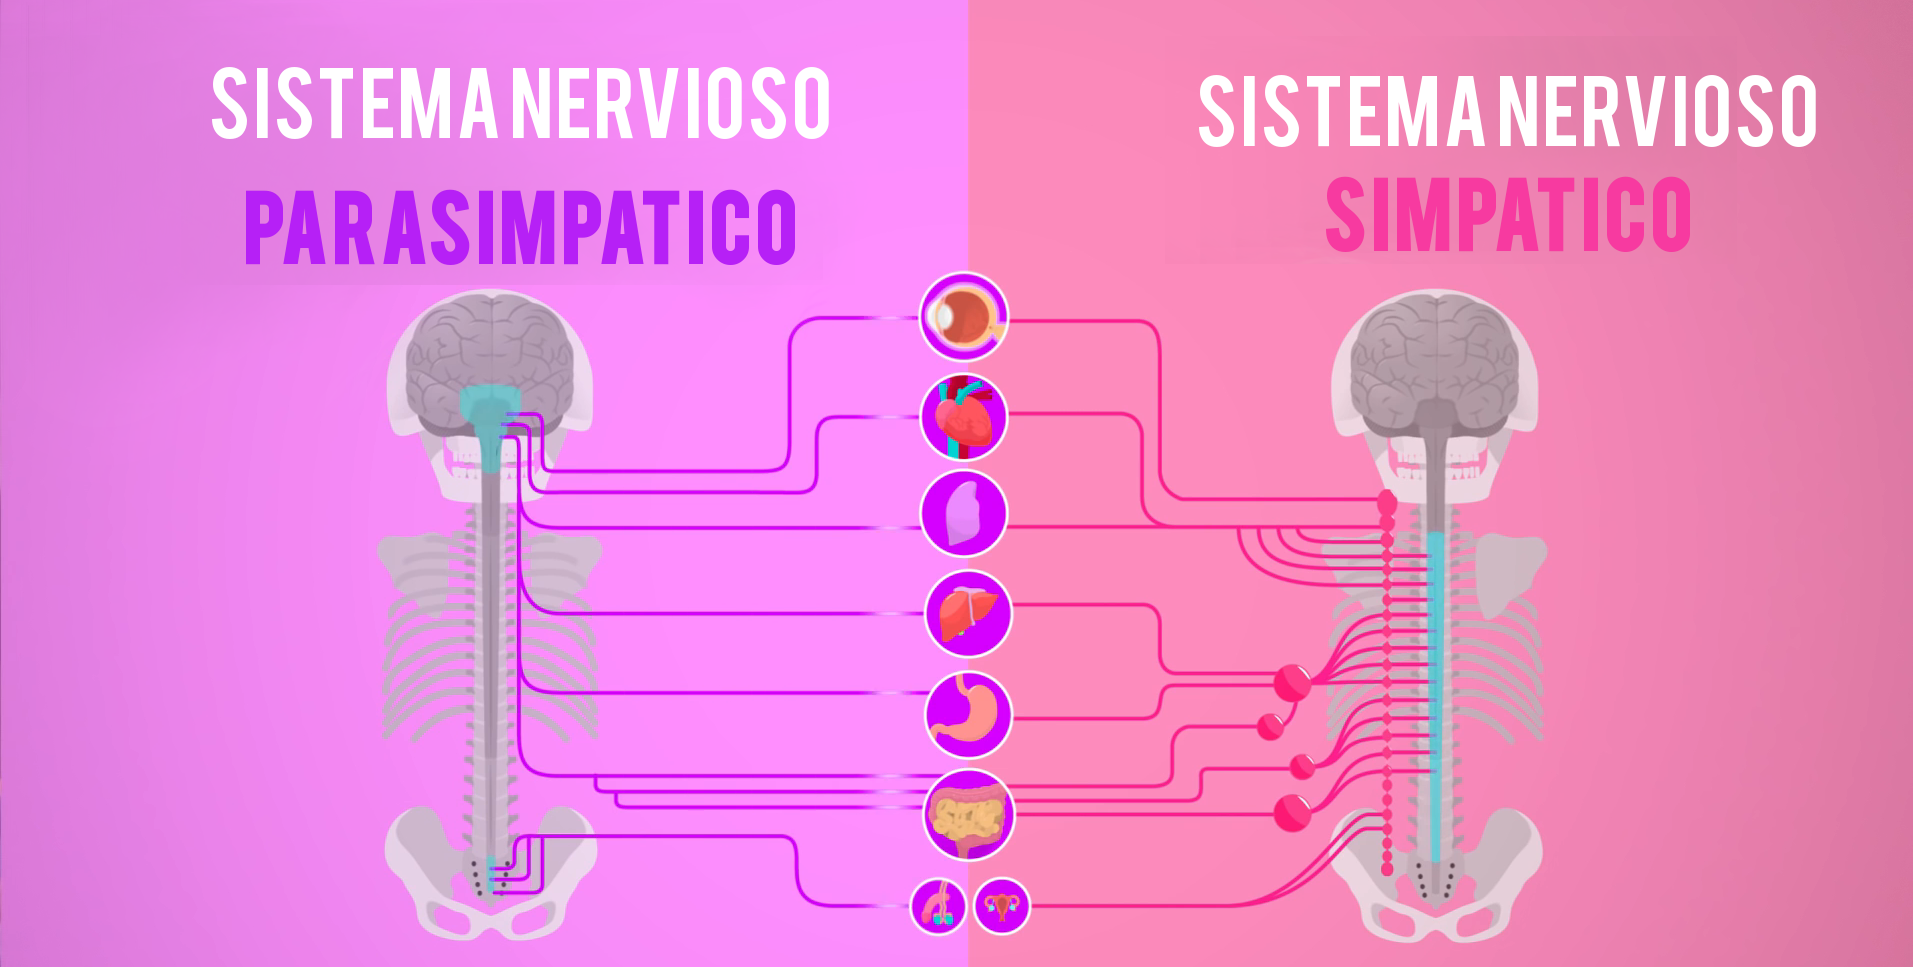
\includegraphics[width=160mm,height=80mm]{./Figures/img_snc}} 
	\caption{El sistema Aut\'onomo central (Crash Course A\&P \#13) \label{fig:modeloSNP}}
\end{figure}

Los efectos de la ansiedad se manifestan (entre otros fen\'omenos) en el ritmo card\'iaco, respiraci\'on y sudoraci\'on. Los cuales son controlados por el SAC. Normalmente, el individuo no tiene control sobre los cambios en sus funciones corporales. Algunos de estos cambios, como la sudoraci\'on y el ritmo card\'iaco pueden ser cuantificados por medio de sensores. A continuaci\'on se explican algunas se\~nales de estos cambios usadas para detectar la ansiedad.

	\subsection{Respuesta Galv\'anica de la Piel (GSR)}\label{secc:gsr}
	Uno de los efectos que la ansiedad causa sobre el cuerpo es la sudoraci\'on. El sudor est\'a formado mayormente por agua y minerales, y ayuda a mantener la temperatura corporal. Un efecto secundario de la presencia del sudor es el cambio en la conductividad el\'ectrica de la piel, siendo esta definida como \textit{``la facilidad que ofrece un material al paso de la corrente el\'ectrica''}. Esta capacidad de conductividad es denotada por la unidad del sistema internacional \textit{Siemen ($S$)}. La unidad $S$ est\'a definida por: $S = \Omega^{-1} = \dfrac{A}{V}$. Donde $\Omega$ es el ohm, $A$ es el amperio y $V$ es el voltio. Debido a que los valores de las mediciones son comunmente muy peque\~nas, las mediciones son denotadas por el prefijo ``micro'' ($\mu$).
	\begin{figure}[h]
		\centering
		\subfigure[]{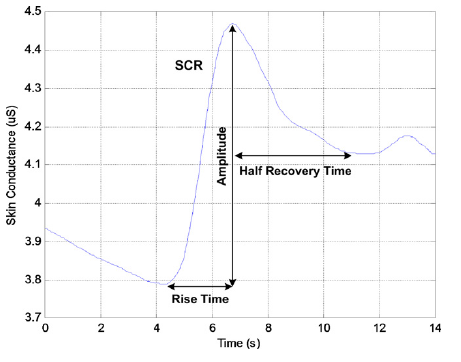
\includegraphics[width=100mm,height=80mm]{./Figures/img_gsr}} 
		\caption{Se\~nal t\'ipica de GSR. El punto de levantamiento est\'a denotado por el c\'irculo de color amarillo. La amplitud por la l\'inea roja y el punto de recuperaci\'on media por la cruz magneta. \label{fig:GSRsignal}}
	\end{figure}

	La se\~nal de GSR se encuentra compuesta por dos partes: Un componente base y un componente t\'onico \citep{Katsis2011261}. El componente base corresponde a un nivel promedio sin un est\'imulo en concreto, mientras que el componente t\'onico es la reacci\'on a un est\'imulo. La figura ~\ref{fig:GSRsignal} ejemplifica ambos componentes. Los picos durante el componente t\'onico tiene las siguientes caracter\'isticas:

\begin{itemize}
        \item{\textbf{Tiempo de Levantamiento del pico:}} Es el tiempo que tarda la se\~nal en alcanzar el punto m\'aximo (pico) en el segmento.
        \item{\textbf{Amplitud del pico:}} Es la distancia que existe entre el punto de levantamiento del pico hasta el punto de valor m\'aximo del pico.
        \item{\textbf{Tiempo de media recuperac\'on :}} Es el tiempo que tarda la se\~nal en disminuir la mitad del valor de la amplitud del pico.
\end{itemize}


	\subsection{Se\~nales relacionadas con el coraz\'on}\label{secc:hearthrate}
	Las se\~nales relacionadas con el coraz\'on se utilizan ampliamente como indicadores principales en estudios de detecci\'on de ansiedad y estr\'es \citep{Sharma20121287}. A continuaci\'on se describen algunas de ellas:
	\begin{itemize}
		\item \textit{Ritmo Card\'iaco (HR):} Se define como el n\'umero de latidos por minuto (BPM).
		\item \textit{Intervalo entre latidos (IBI):} Se define como el tiempo en segundos entre un latido y otro. Esta se\~nal est\'a directamente relacionada con el ritmo card\'iaco. Entre menor sea el valor de IBI, mayor ser\'a el valor del HR.
	\end{itemize}
	\subsection{Electroencefalograma (EEG)}\label{secc:eeg}
	Un electroencefalograma permite medir la diferencia en voltaje entre dos puntos del cerebro. El EEG consiste en el estudio y grabaci\'on de estas se\~nales ele\'ctricas \citep{tatum2014handbook}. Las se\~nales el\'ectricas son creadas cuando cargas el\'ectricas se mueven dentro del sistema nervioso central. Existen dos tipos de instrumentos para EEG. Los Intracraneales que permiten medir la energ\'ia de neuronas espec\'ificas por medio de dispositivos injertados en el cerebro, y los extracraneales, sensores puestos en el cuero cabelludo. El desarrollo de dispositivos extracraneales en los \'ultimos a\~nos ha abierto la posibilidad de realizar mediciones de EEG no intrusivas y a bajo costo.
\section{Instrumentos tradicionales para la medici\'on de la ansiedad}
        En psicolog\'ia existen diversos instrumentos que permiten detectar la ansiedad. Algunos de los cuestionarios existentes son:
        \begin{itemize}

		\item Escala de \'indice de ansiedad de Hamilton \textit{Hamilton Anxiety Rating Scale (HAM-A):}

			La prueba HAM-A fu\'e una de las primeras escalas desarrolladas para medir la severidad de los s\'intomas de la ansiedad, y sigue siendo ampliamente usada para fines cl\'inicos y de investigaci\'on. Consiste en una prueba de 14 reactivos, cada uno definido por una serie de s\'intomas \citep{PAPT467}.
		\item Escala de ansiedad autocalificada de Zung \textbf{Zung Self-Rating Anxiety Scale (SAS):}

			La prueba SAS es una de herramienta de 20 frases relacionadas con las experiencias sentidas durante los d\'ias anteriores \citep{Zung1971371}. Algunas de las frases son: \textit{``He sentido mi coraz\'on latir r\'apido.''}, \textit{``Me he sentido mas nervioso y ansioso de lo normal.''} y \textit{``He sentido miedo sin una raz\'on aparente''}. Cada respuesta tiene un valor que var\'ia desde 1 hasta 4, donde 1 representa ``Nada o poco del tiempo'' y 4 ``Casi todo el tiempo''. La puntuaci\'on final permite diferenciar entre 3 posibles niveles de ansiedad: \textit{``Dentro del rango normal''}, \textit{``De ansiedad m\'inima a moderada''}, \textit{``Ansiedad severa''}, \textit{``Ansiedad extrema''}.
		\item El inventario de ansiedad estado-rasgo \textbf{The State-Trait Anxiety Inventory (STAI):}
			La prueba STAI permite medir mediante auto-reportado la presencia y severidad de los s\'intomas de la ansiedad y la tendencia a ser ansioso\citep{julian2011measures}. Consiste de 40 reactivos, los cuales hacen preguntas de como se siente el sujeto en el momento. Las posibles respuestas son: 1) Para nada, 2) Un poco, 3) Moderadamente, 4) Mucho. Los rangos de la puntuaci\'on se interpretan en 3 posibles niveles de ansiedad: \textit{``Nada de ansiedad''}, \textit{``Ansiedad moderada''} y \textit{``Ansiedad extrema''}

		\item Escala de ansiedad subjetiva autocalificada \textbf{Subjective Self-raiting Anxiety Scale (SUDS):}
			La escala SUDS permite medir el nivel de ansiedad por medio de una sola escala \citep{wolpe1973practice}. La escala var\'ia desde 0 a 100, con pasos de 10. Cada nivel tiene una descripci\'on asociada como: \textit{``20, Ansiedad M\'inima.''}, \textit{``50, Ansiedad moderada. Me siento inc\'omodo''} y \textit{``100, La ansiedad mas grande que he sentido en mi vida''}. La ventaja sobre otras escalas es que permite obtener el nivel de ansiedad casi instant\'aneamente, haciendola \'util en situaciones donde es necesario monitorear el nivel de ansiedad constantemente.
        \end{itemize}


\section{C\'omputo vestible}\label{secc:dementia}
El c\'omputo vestible nos permite llevar computadoras con nosotros de la misma manera que llevamos la ropa puesta. Al ``vestir'' un dispositivo, el usuario tiene acceso a una computadora que es capaz de monitorearlo a \'el y a su entorno por medio de sensores. Los sensores pueden medir par\'ametros tales como el movimiento del usuario, su posici\'on, intensidad de luz, ruido, im\'agenes de su ambiente, ritmo card\'iaco, capacidad conductiva de la piel, distancias, actividad cerebral, entre otros. Debido a la cercania con el usuario, se pueden hacer monitoreos constantes y mas precisos que con los sistemas tradicionales. Esta cualidad permite dise\~nar sistemas que pueden ayudar en las tareas de la vida cotidiana.

El uso de c\'omputo vestible abre la posibilidad de detectar la ansiedad por medio de las se\~nales fisiol\'ogicas del usuario.

\section{Trabajo previo en detecci\'on autom\'atica de ansiedad}
El c\'omputo afectivo es una rama relativamente nueva de las ciencias de la computaci\'on. Su finalidad es que la computadora sea capaz de reconocer o emitir emociones humanas \citep{picard1997affective}. Existen trabajos que utilizan el c\'omputo afectivo para detectar la ansiedad. Estos estudios, por lo general toman un enfoque parecido al del reconocimiento de patrones, el cual se basa en tres diferentes fases: \textit{Captura de datos y pre-procesamiento}, \textit{Extracci\'on de caracter\'isticas} y \textit{Clasificaci\'on}. (Ver Figura ~\ref{fig:anxiDetection}). 

\begin{figure}[h]
	\centering
	\subfigure[]{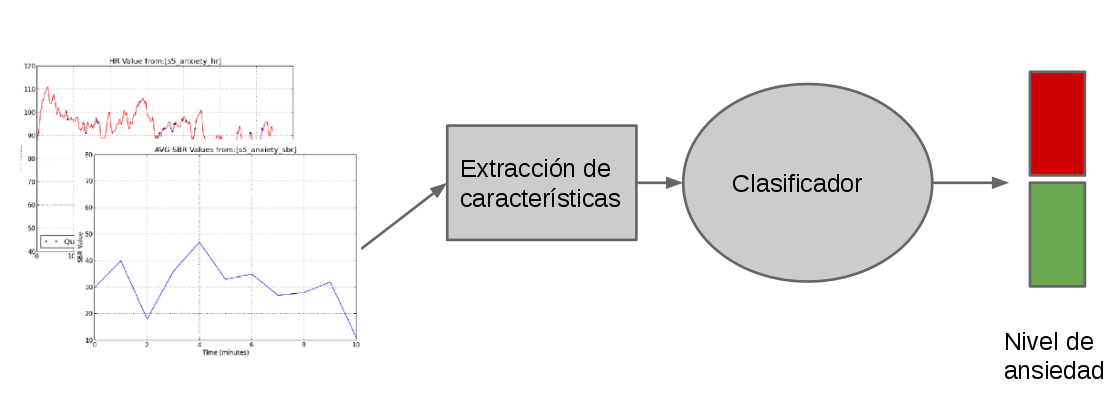
\includegraphics[width=160mm,height=140mm,keepaspectratio]{./Figures/img_anxietydetection}} 
	\caption{Fases comunmente usadas en el reconocimiento de emociones} \label{fig:anxiDetection}
\end{figure}

Normalmente estas intervenciones implementan alguna t\'ecnica para inducir ansiedad. Una de las t\'ecnicas usada es aplicando pruebas mentales al participante \citep{rani2007anxiety} o por medio de situaciones simuladas en un entorno virtual en tercera dimensi\'on (Repetto \textit{et al.}, 2013; Handouzi \textit{et al.}, 2014) para luego medir las respuestas de sus se\~nales fisiol\'ogicas. Estos estudios toman en cuenta tambi\'en tiempos de relajaci\'on inicial y periodos de descanso entre pruebas, facilitando la diferenciaci\'on entre los estados emocionales con resultados mayores al 75\% en precis\'on.

Estos estudios se realizan bajo entornos controlados, por lo que la intensidad y frecuencia de los estresores pueden cambiar para cada prueba. Sin embargo, los entornos naturales donde se genera la ansiedad tienden a ser mas impredecibles y din\'amicos. Otras intervenciones se realizan en entornos simulados de oficina para detectar el estr\'es causado por cargas cognitivas \citep{Cinaz13} con resultados de hasta 69.8\% de precisi\'on.

En la actualidad, no existen intervenciones para la detecci\'on de ansiedad en cuidadores en situaciones de laboratorio ni naturalistas.
\section{M\'aquinas de soporte vectorial (SVM)}
La \'utlima fase de la detecci\'on de ansiedad es usualmente la implementaci\'on de alguna t\'ecnica de aprendizaje de m\'aquina. Un modelo tradicional es el de la m\'aquina de soporte vectorial \footnote{Support Vector Machine}. La finalidad de la SVM es el resolver un problema de clasificaci\'on cuando se tienen $n$ muestras de al menos dos clases. Esto se resuelve calculando el hiperplano \'optimo que separe las clases diferentes. La figura ~\ref{fig:svm} muestra el espacio de muestras y el hiperplano \'optimo. Los planos paralelos son los vectores de soporte que ayudan a separar las clases con seguridad. La SVM se puede utilizar para el reconocimiento de ansiedad si cuantificamos las caracteristicas de los eventos de ansiedad y los proyectamos en un espacio de n\'umeros reales.
\begin{figure}[h]
	\centering
	\subfigure[]{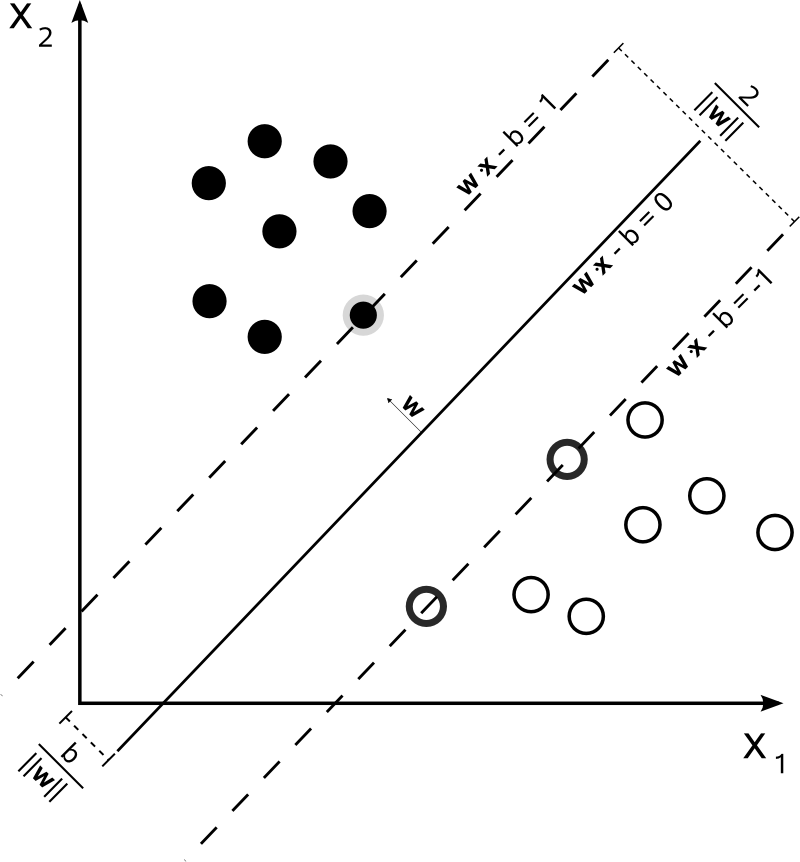
\includegraphics[width=80mm,keepaspectratio]{./Figures/img_svm}} 
	\caption{Ejemplo del funcionamiento de la m\'aquina de soporte vectorial} \label{fig:svm}
\end{figure}

\section{Conclusi\'on}\label{secc:conclution}
La disponibilidad actual del c\'omputo vestible y su capacidad de capturar se\~nales del cuerpo constantemente abren la posibilidad de cuantificar estados mentales que tradicionalmente requieren tiempo e interpretaci\'on de un especialista para medir. La detecci\'on de ansiedad podr\'ia dar lugar al desarrollo de aplicaciones que sugieran al cuidador estrategias de afrontamiento para reducir la ansiedad y mejorar su bienestar general. Sin embargo, el capturar datos de situaciones de ansiedad en situaciones naturalistas y su an\'alisis representa un reto. En el siguiente cap\'itulo, se explica el desarrollo de un estudio de usuario para obtener datos de cuidadores haciendo uso del c\'omputo vestible.
\newpage
%%=====================================================
